\section{Descripción de los juegos}

Los algoritmos fueron probados en juegos diferente en forma normal. Estos juegos son de suma cero para dos persona, por lo tanto es suficiente con mostrar el pago para el jugador $1$ para que esté bien definido. Además, cualquier juego con estas características puede modelarse como un problema de programación lineal y resolverse mediante procedimientos destinados para esto. Cada juego es descrito a continuación, con su matriz de pagos y problema de programación lineal asociado con su solución respectiva, en los casos que los juegos sean lo suficientemente pequeño para mostrarlos.

\subsection{Matching pennies}
En este juego cada jugador tiene una moneda y selecciona cara o sello de forma secreta. Si las elecciones son gana el jugador $1$, en caso contrario gana el jugador $2$. La matriz de pagos de este juego se muestra en la Tabla \ref{table:pagos-matching-pennies}
\begin{table}[ht]
\begin{center}
\caption[Tabla de pagos del juego matching pennies]{Tabla de pagos del juego \textit{matching pennies}}
\label{table:pagos-matching-pennies}
\begin{tabular}{ c | c | c |}
 & cara & sello  \\ \hline
 cara  &  1 & -1 \\ \hline
 sello & -1 &  1 \\ \hline
\end{tabular}
\end{center}
\end{table}

El problema de programación lineal asociado es el siguiente
\begin{equation}
\begin{array}{r r r r r r r r}
\max  & z &  & & & & &\\
\text{s.a.}  
&   &   & x_1  & + & x_2 & = & 1 \\
& z & - & x_1  & + & x_2 & \leq & 0 \\
& z & + & x_1  & - & x_2 & \leq & 0 \\
&   &   & x_1, &   & x_2 & \geq & 0
\end{array}
\end{equation}
Cuya solución primal viene dada por $(z*, x_1^*, x_2^*) = (0, \frac{1}{2}, \frac{1}{2})$ y su solución dual por $(w^*, y^*_1, y^*_2) = (0, \frac{1}{2}, \frac{1}{2})$. Luego el equilibrio de Nash se obtiene cuando ambos jugadores eligen cara o sello con probabilidad $\frac{1}{2}$ y el valor del juego es igual a $0$.

\subsection{Piedra, Papel o Tijeras}
Este juego es descrito en la sección \ref{section:forma-normal} y su matriz de pago se muestra en la Tabla \ref{table:pago-RPS}. El problema de programación lineal asociado es el siguiente:
\begin{equation}
\begin{array}{r r r r r r r r r r}
\max  & z &  & & & & &\\
\text{s.a.}  
&   &   & x_1  & + & x_2  & + & x_3 & =    & 1 \\
& z &   &      & + & x_2  & - & x_3 & \leq & 0 \\
& z & - & x_1  &   &      & + & x_3 & \leq & 0 \\
& z & + & x_1  & - & x_2  &   &     & \leq & 0 \\
&   &   & x_1, &   & x_2, &   & x_3 & \geq & 0
\end{array}
\end{equation}

Y la solución primal y dual de este problema son $(z^*, x_1^*, x_2^*, x_3^*) = (0, \frac{1}{3}, \frac{1}{3}, \frac{1}{3})$ y $(w^*, y_1^*, y_2^*, y_3^*) = (0, \frac{1}{3}, \frac{1}{3}, \frac{1}{3})$, respectivamente. Luego, el equilibrio de Nash se obtiene cuando ambos jugadores eligen cada una de las acciones con probabilidad igual a $\frac{1}{3}$.

\subsection{Ficha vs Dominó}
Cada jugador tiene un tablero de tamaño $2\times 3$, el primer jugador tiene una ficha de dominó (que ocupa dos casillas con un lado en común) que puede colocar de $7$ formas diferentes, cada forma es mostrada en la figura \ref{fig:posiciones-domino}, con su respectiva eiqueta. El segundo jugador posee una ficha que ocupa una sóla casilla de su tablero y la ubica en una de las $6$ casillas, las cuales se numeran en la Figura \ref{fig:posiciones}. Luego se superponen los tableros y si la ficha es cubierta por el dominó entonces el segundo jugador gana, en caso contrario gana el primer jugador \cite[p. 237]{bib:pl-chvatal}.

\begin{figure}[hbt!]
\caption{Posibles posiciones de la ficha de dominó}
\label{fig:posiciones-domino}
\centering
\includegraphics[width=1\textwidth]{figuras/posiciones-domino.png}
\end{figure}

\begin{figure}[hbt!]
\caption{Posibles posiciones de la ficha del segundo jugador}
\label{fig:posiciones}
\centering
\includegraphics[width=0.4\textwidth]{figuras/posiciones.png}
\end{figure}

\begin{table}[hbt]
\begin{center}
\caption{Matriz de pagos del juego Ficha vs Dominó}
\label{table:pagos-domino}
\begin{tabular}{ c | c | c | c | c | c | c |}
  &  1 &  2 &  3 &  4 &  5 &  6 \\ \hline
A & -1 & -1 &  1 &  1 &  1 &  1 \\ \hline
B &  1 &  1 &  1 & -1 & -1 &  1 \\ \hline
C &  1 & -1 & -1 &  1 &  1 &  1 \\ \hline
D &  1 &  1 &  1 &  1 & -1 & -1 \\ \hline
E & -1 &  1 &  1 & -1 &  1 &  1 \\ \hline
F &  1 & -1 &  1 &  1 & -1 &  1 \\ \hline
G &  1 &  1 & -1 &  1 &  1 & -1 \\ \hline
\end{tabular}
\end{center}
\end{table}

El problema de programación lineal asociado es:
\begin{equation}
\begin{array}{r r r r r r r r r r r r r r r r r r}
max        &z& &   & &   & &   & &   & &   & &   & &   &      & \\
\text{s. a}
	& & &x_1&+&x_2&+&x_3&+&x_4&+&x_5&+&x_6&+&x_7& =    &1 \\
    &z&+&x_1&-&x_2&-&x_3&-&x_4&+&x_5&-&x_6&-&x_7& \leq &0 \\
    &z&+&x_1&-&x_2&+&x_3&-&x_4&-&x_5&+&x_6&-&x_7& \leq &0 \\
    &z&-&x_1&-&x_2&+&x_3&-&x_4&-&x_5&-&x_6&+&x_7& \leq &0 \\
    &z&-&x_1&+&x_2&-&x_3&-&x_4&+&x_5&-&x_6&-&x_7& \leq &0 \\
    &z&-&x_1&+&x_2&-&x_3&+&x_4&-&x_5&+&x_6&-&x_7& \leq &0 \\
    &z&-&x_1&-&x_2&-&x_3&+&x_4&-&x_5&-&x_6&+&x_7& \leq &0 \\
    & & &x_1,&&x_2,&&x_3,&&x_4,&&x_5,&&x_6,&&x_7,&\geq &0 \\
\end{array}
\end{equation}

Este problema no tiene solución única (lo que implica que el juego no tiene un equilibrio de Nash único), una solución viene dada por $(z^*, x^*_1, x^*_2, x^*_4, x^*_5, x^*_6, x^*_6, x^*_7) = (\frac{1}{3}, \frac{1}{3}, \frac{1}{3}, 0, 0, 0, 0, \frac{1}{3})$ y $(w^*, y^*_1, y^*_2, y^*_3,  y^*_4, y^*_5, y^*_6) = (\frac{1}{3}, \frac{1}{3}, 0, \frac{1}{3}, 0, \frac{1}{3}, 0)$, esta solución corresponde a la estrategia en la que el jugador $1$ elige las posiciones A, B y G con probabilidad $\frac{1}{3}$ cada una, y el jugador $2$ elige las posiciones $1$, $3$, y $5$ con probabilidad $\frac{1}{3}$ cada una.

\subsection{Coronel Blotto}
En este juego cada uno de los jugadores tiene $S$ soldados en total, y cada soldado puede ser asignado a uno de los $N$ campos de batalla. Cualquier número de soldados puede ser colocado en cualquier campo, incluyendo el cero. Un jugador obtiene un campo de batalla si asigna más soldados que su oponente en ese campo de batalla. El juego es ganado por el jugador que obtenga un mayor número de campos y su pago es igual a la diferencia entre el número de campos obtenidos por cada uno de los jugadores \cite{bib:introductionCFR}.

Formalmente el juego puede ser descrito de la siguiente manera. Cada jugador debe elegir $N$ números enteros, digamos $(a_1, a_2, ..., a_N)$ y $(b_1, b_2, ..., b_N)$, para el jugador $1$ y $2$ respectivamente, tales que $a_1 + a_2 + ... + a_N = S$ y $b_1 + b_2 + ... + b_N = S$, con $N < S$, donde $a_i$ y $b_i$ es la cantidad de soldados ubicados el $i$-ésimo campo por el primer y segundo jugador, respectivamente. Para estas distribuciones, la ganancia del jugador $1$ viene dada por:
\begin{alignat}{1}
|\{ 1 \leq i \leq N : a_i > b_i\}| - |\{ 1 \leq i \leq N : a_i < b_i\}|
\end{alignat}

Este juego depende de dos parámetros: el número de soldados $S$ y el número de campos de batallas $N$, por lo que la matriz de pagos no es constante y por eso no es presentada como en los juegos anteriores. La matriz para de un juego con $S$ soldados y $N$ es una matriz cuadrada de tamaño $\binom{N+S-1}{S-1}$.

\subsection{Kunh Poker}
Este juego fue descrito en la sección \ref{section:kuhn-poker}. A diferencia de los juegos anteriores, es un juego secuencial, por lo que su representación natural es en forma extensiva. Sin embargo, como se mostró en la sección \ref{section:normal-extensiva}, todo juego en forma extensiva puede ser representado en forma normal, por lo que se pueden aplicar los algoritmos a al forma normal correspondiente.

En este juego, el jugador $2$ tiene una ganancia esperada de $\frac{1}{18}$ por mano, como se prueba en \cite{bib:kuhn-poker}. Además, el primer jugador tiene infinitas estrategias óptimas, las cuales pueden ser representadas por la elección de un parámetro $\alpha \in [ 0, \frac{1}{3} ]$. Una vez elegido este parámetro, en la primera jugada del primer jugador, este apuesta con probabilidad $\alpha$ cuando su carta tenga el número $1$, apuesta con una probabilidad $3 \alpha$ cuando tiene el número $3$ y siempre pasa cuando tiene el número $2$. Si el primer jugador tiene un segundo turno, debe pasar siempre que tenga el número $1$, apostar cuando tiene el número $3$, y en el caso que tenga el número $2$ debe apostar con probabilidad $\alpha + \frac{1}{3}$.

El segundo jugador tiene una única estrategia mixta óptima: apostar siempre que tenga el número $3$. Cuando tenga el número $1$, pasar siempre que el primer jugador haya apostado y apostar con probabilidad $\frac{1}{3}$ en caso contrario. Cuando tenga el número $2$, debe pasar cuando el oponente haya pasado previamente y apostar con probabilidad $\frac{2}{3}$ en caso contrario. La figura \ref{fig:kunh-poker-estrategias} muestra el árbol con las distribuciones de probabilidad de las estrategias previamente descritas en cada uno de los nodos alcanzables en el juego.

\begin{figure}[ht]
\begin{center}
\caption{Equilibrio de Nash del juego de Kunh poker}
\label{fig:kunh-poker-estrategias}
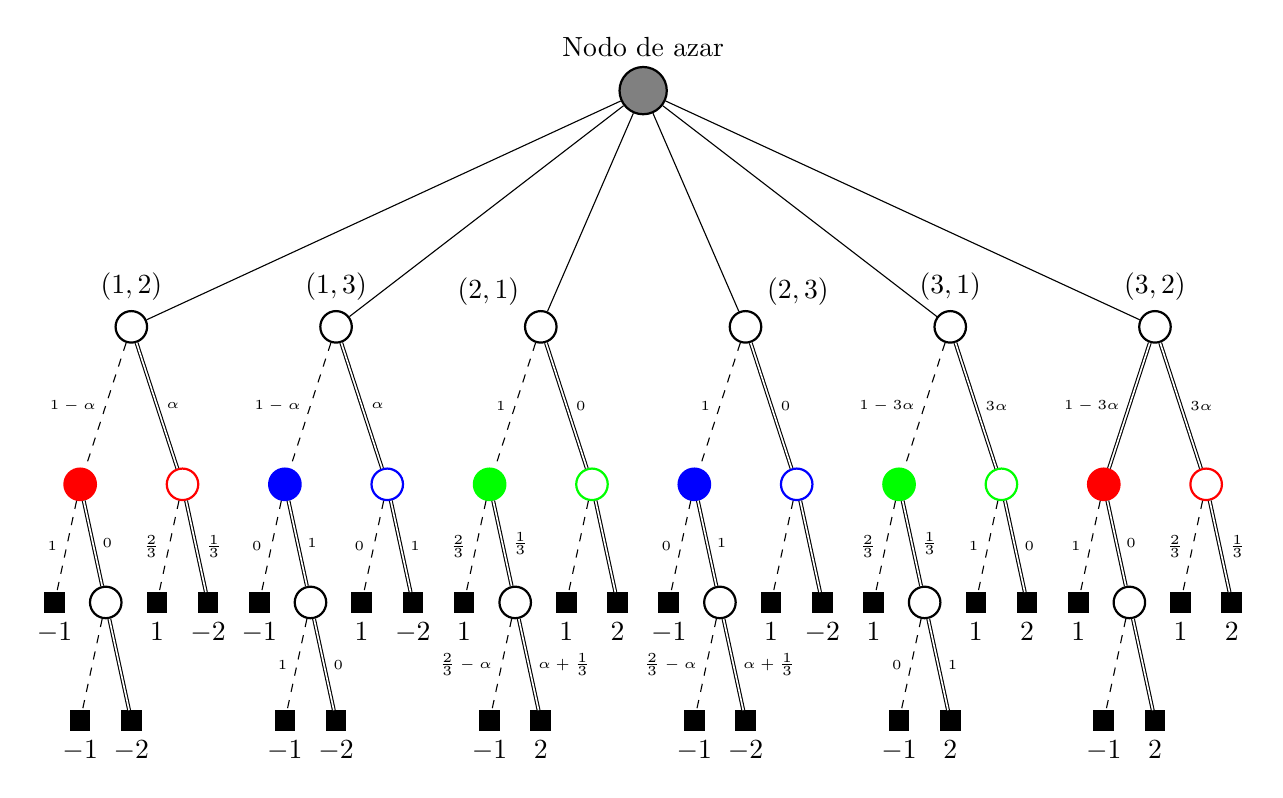
\begin{tikzpicture}[
chance/.style={circle, draw=black, fill=gray, thick, minimum size = 6mm},
player1/.style={circle, draw=black, solid, thick, minimum size = 4mm},
player2/.style={circle, thick, minimum size=4mm},
terminal/.style={rectangle, draw=black, solid, fill=black, thick, minimum size=2mm},
level 1/.style={sibling distance=26mm, level distance=30mm},
level 2/.style={sibling distance=13mm, level distance=20mm},
level 3/.style={sibling distance=6.5mm, level distance=15mm},
]
\node[chance] [label=above:{Nodo de azar}] {} {
	child {node [player1] (P1) [label=above:{$(1, 2)$}]{}
		child { node [player2] [draw=red, fill=red] {} 
				child { node [terminal] [label=below:{$-1$}] {}
						edge from parent [dashed] node [left, draw=none] {\tiny{$1$}} {} }
				child { node [player1] (A) {} 
						child { node [terminal] [label=below:{$-1$}] {}
								edge from parent [dashed] {} }
						child { node [terminal] [label=below:{$-2$}] {} 
								edge from parent [solid, double] {} }
						edge from parent [solid, double] node [right, draw=none] {\tiny{$0$}}  {}
				}
				edge from parent [dashed] node [left, draw=none] {\tiny{$1-\alpha$}}  {}
		}
		child { node [player2] [draw=red] {} 
				child { node [terminal] [label=below:{$1$}] {}
						edge from parent [dashed] node [left, draw=none] {\tiny{$\frac{2}{3}$}} {} }
				child { node [terminal] [label=below:{$-2$}] {}
						edge from parent [solid, double] node [right, draw=none] {\tiny{$\frac{1}{3}$}} {} }
				edge from parent [solid, double] node [right, draw=none] {\tiny{$\alpha$}}{}
		}
	}
	child {node [player1] (P2) [label=above:{$(1, 3)$}]{}
		child { node [player2] [draw=blue, fill=blue] {} 
				child { node [terminal] [label=below:{$-1$}] {}
						edge from parent [dashed] node [left, draw=none] {\tiny{$0$}} {} }
				child { node [player1] (B) {} 
						child { node [terminal] [label=below:{$-1$}] {}
								edge from parent [dashed] node [left, draw=none] {\tiny{$1$}} {} }
						child { node [terminal] [label=below:{$-2$}] {}
								edge from parent [solid, double] node [right, draw=none] {\tiny{$0$}} {} }
						edge from parent [solid, double] node [right, draw=none] {\tiny{$1$}} {}
				}
				edge from parent [dashed] node [left, draw=none] {\tiny{$1-\alpha$}} {}
		}
		child { node [player2] [draw=blue] {} 
				child { node [terminal] [label=below:{$1$}] {}
						edge from parent [dashed] node [left, draw=none] {\tiny{$0$}} {} }
				child { node [terminal] [label=below:{$-2$}] {}
						edge from parent [solid, double] node [right, draw=none] {\tiny{$1$}} {} }
				edge from parent [solid, double] node [right, draw=none] {\tiny{$\alpha$}} {}
		}
	}
	child {node [player1] (P3) [label=135:{$(2, 1)$}]{}
		child { node [player2] [draw=green, fill=green] {} 
				child { node [terminal] [label=below:{$1$}] {}
						edge from parent [dashed] node [left, draw=none] {\tiny{$\frac{2}{3}$}} {} }
				child { node [player1] (C) {} 
						child { node [terminal] [label=below:{$-1$}] {}
								edge from parent [dashed] node [left, draw=none] {\tiny{$\frac{2}{3}-\alpha$}} {} }
						child { node [terminal] [label=below:{$2$}] {} 
                        		edge from parent [solid, double] node [right, draw=none] {\tiny{$\alpha+\frac{1}{3}$}} {} }
						edge from parent [solid, double] node [right, draw=none] {\tiny{$\frac{1}{3}$}} {}
				}
				edge from parent [dashed] node [left, draw=none] {\tiny{$1$}} {}
		}
		child { node [player2] [draw=green] {} 
				child { node [terminal] [label=below:{$1$}] {}
						edge from parent [dashed] {} }
				child { node [terminal] [label=below:{$2$}] {}
						edge from parent [solid, double] {} }
				edge from parent [solid, double] node [right, draw=none] {\tiny{$0$}} {}
		}
	}
	child {node [player1] (P4) [label=45:{$(2, 3)$}]{}
		child { node [player2] [draw=blue, fill=blue]{} 
				child { node [terminal] [label=below:{$-1$}] {}
						edge from parent [dashed] node [left, draw=none] {\tiny{$0$}} {} }
				child { node [player1] (D) {} 
						child { node [terminal] [label=below:{$-1$}] {}
								edge from parent [dashed] node [left, draw=none] {\tiny{$\frac{2}{3}-\alpha$}} {} {} }
						child { node [terminal] [label=below:{$-2$}] {}
								edge from parent [solid, double] {} node [right, draw=none] {\tiny{$\alpha+\frac{1}{3}$}} {} }
						edge from parent [solid, double] node [right, draw=none] {\tiny{$1$}} {}
				}
				edge from parent [dashed] node [left, draw=none] {\tiny{$1$}} {}
		}
		child { node [player2] [draw=blue] {} 
				child { node [terminal] [label=below:{$1$}] {}
						edge from parent [dashed] {} }
				child { node [terminal] [label=below:{$-2$}] {}
						edge from parent [solid, double] {} }
				edge from parent [solid, double] node [right, draw=none] {\tiny{$0$}} {}
		}
	}
	child {node [player1] (P5) [label=above:{$(3, 1)$}]{}
		child { node [player2] [draw=green, fill=green] {} 
				child { node [terminal] [label=below:{$1$}] {}
						edge from parent [dashed] node [left, draw=none] {\tiny{$\frac{2}{3}$}} {} }
				child { node [player1] (E) {} 
						child { node [terminal] [label=below:{$-1$}] {}
								edge from parent [dashed] node [left, draw=none] {\tiny{$0$}} {} }
						child { node [terminal] [label=below:{$2$}] {}
								edge from parent [solid, double] node [right,draw=none] {\tiny{$1$}} {} }
						edge from parent [solid, double] node [right, draw=none] {\tiny{$\frac{1}{3}$}} {}
				}
				edge from parent [dashed] node [left, draw=none] {\tiny{$1-3 \alpha$}} {}
		}
		child { node [player2] [draw=green] {} 
				child { node [terminal] [label=below:{$1$}] {}
						edge from parent [dashed] node [left, draw=none] {\tiny{$1$}} {} }
				child { node [terminal] [label=below:{$2$}] {}
						edge from parent [solid, double] node [right, draw=none] {\tiny{$0$}} {} }
				edge from parent [solid, double] node [right, draw=none] {\tiny{$3 \alpha$}} {}
		}
	}
	child {node [player1] (P6) [label=above:{$(3, 2)$}]{}
		child { node [player2]  [draw=red, fill=red] {} 
				child { node [terminal] [label=below:{$1$}] {}
						edge from parent [dashed] node [left, draw=none] {\tiny{$1$}} {} }
				child { node [player1] (F) {} 
						child { node [terminal] [label=below:{$-1$}] {}
								edge from parent [dashed] {}}
						child { node [terminal] [label=below:{$2$}] {}
								edge from parent [solid, double] {} }
						edge from parent [solid, double] node [right, draw=none] {\tiny{$0$}} {}
				}
				edge from parent [solid, double] node [left, draw=none] {\tiny{$1-3\alpha$}} {}
		}
		child { node [player2]  [draw=red] {} 
				child { node [terminal] [label=below:{$1$}] {}
						edge from parent [dashed] node [left, draw=none] {\tiny{$\frac{2}{3}$}} {} }
				child { node [terminal] [label=below:{$2$}] {}
						edge from parent [solid, double] node [right, draw=none] {\tiny{$\frac{1}{3}$}} {} }
				edge from parent [solid, double] node [right, draw=none] {\tiny{$3\alpha$}} {}
		}
	}
};
\end{tikzpicture}
\end{center}
\end{figure}
